\documentclass[../main.tex]{subfiles}
\graphicspath{{\subfix{../images/}}}
\begin{document}

\subsubsection{Contrast and Sharpness}

\begin{figure}[h!]
  \centering
  \begin{subfigure}[b]{0.2\linewidth}
    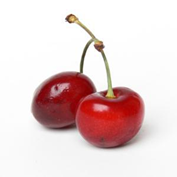
\includegraphics[width=\linewidth]{original.png}
  \end{subfigure}
  \begin{subfigure}[b]{0.2\linewidth}
    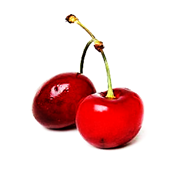
\includegraphics[width=\linewidth]{edited.png}
  \end{subfigure}
  \caption{Cherry with increased contrast and sharpness}
  \label{fig:contrast-edit}
\end{figure}

In Figure \ref{fig:contrast-edit}, the image with contrast and sharpness increased on the right. It can be seen that the cherry shape has become more clear and can be seen even against the second cherry. This change helps the model see shapes of the fruit clearer which could make it easier for the model to classify the images. 


\end{document}